\documentclass[11pt,a4paper]{scrartcl}

\usepackage[a4paper,margin=2.6cm]{geometry}
\usepackage[T1]{fontenc}
\usepackage[utf8]{inputenc}
\IfFileExists{lmodern.sty}{\usepackage{lmodern}}{\usepackage{mathpazo}}% font vettoriali anche dove manca Latin Modern
\usepackage{amsmath,amssymb}
\usepackage{tikz}
\usetikzlibrary{arrows.meta,angles,quotes,calc,decorations.markings}
\usepackage[most]{tcolorbox}
\usepackage{xcolor}
\usepackage{enumitem}
\usepackage{needspace}

\hyphenpenalty=10000 \exhyphenpenalty=10000 \emergencystretch=4em

% ---------- box "Esercizio" in stile OpenStax ----------
\newtcolorbox{esercizio}[1][]{%
  enhanced,
  breakable,
  colback=white,
  colframe=black,
  boxrule=0.6pt,
  sharp corners,
  left=2mm,right=2mm,top=1.5mm,bottom=1.5mm,
  before skip=6mm, after skip=4mm,
  #1
}

\newenvironment{soluzione}{\par\noindent\textbf{Soluzione ---} }{\par}

% ---------- macro rapide ----------
\newcommand{\un}[1]{\,\mathrm{#1}}
\newcommand{\vm}{\vec m}
\newcommand{\vB}{\vec B}

% ---------- figure riutilizzabili ----------
% superficie piana con normale n e campo B a angolo #1 dalla normale
\newcommand{\figflusso}[1]{%
\begin{center}\begin{tikzpicture}[>=Latex,scale=0.85]
  \draw[fill=gray!12] (0,0)--(3.4,0)--(4.6,1.0)--(1.2,1.0)--cycle;
  \coordinate (O) at (2.3,0.5);
  \draw[->,thick] (O)--++(0,2.0) node[above]{$\hat n$};
  \pgfmathsetmacro{\aB}{90-#1}
  \draw[->,thick,gray!60!black] (O)--++(\aB:2.4) node[right]{$\vB$};
  \draw (O)++(0,1.0) arc (90:\aB:1.0);
  \node at ($(O)+({90-#1/2}:1.28)$) {$\theta$};
  \node[below] at (2.3,-0.1) {superficie $S$};
\end{tikzpicture}\end{center}}

\newcommand{\figcubo}{%
\begin{center}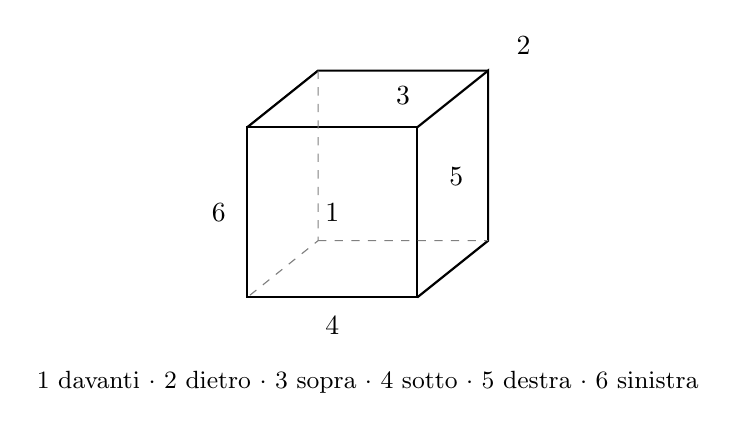
\begin{tikzpicture}[>=Latex,scale=0.9]
  \draw[thick] (0,0) rectangle (2.4,2.4);
  \draw[thick] (2.4,0)--(3.4,0.8)--(3.4,3.2)--(2.4,2.4);
  \draw[thick] (0,2.4)--(1,3.2)--(3.4,3.2);
  \draw[dashed,gray] (1,3.2)--(1,0.8)--(0,0) (1,0.8)--(3.4,0.8);
  \node at (1.2,1.2) {1};   % davanti
  \node at (2.2,2.85) {3};  % sopra
  \node at (2.95,1.7) {5};  % destra
  \node at (-0.4,1.2) {6};  % sinistra
  \node at (1.2,-0.4) {4};  % sotto
  \node at (3.9,3.55) {2};  % dietro
  \node[font=\small] at (1.7,-1.2) {1 davanti $\cdot$ 2 dietro $\cdot$ 3 sopra $\cdot$ 4 sotto $\cdot$ 5 destra $\cdot$ 6 sinistra};
\end{tikzpicture}\end{center}}

\newcommand{\figpannelli}{%
\begin{center}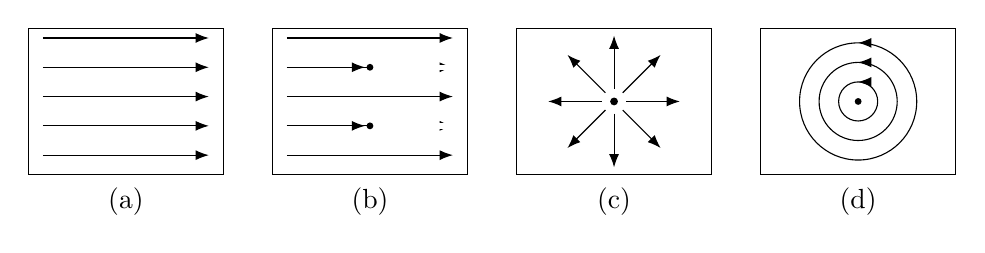
\begin{tikzpicture}[>=Latex,scale=0.62]
  % (a) uniformi
  \begin{scope}
    \draw (0,0) rectangle (4,3);
    \foreach \y in {0.4,1.0,1.6,2.2,2.8} \draw[->] (0.3,\y)--(3.7,\y);
    \node at (2,-0.55) {(a)};
  \end{scope}
  % (b) alcune linee si interrompono
  \begin{scope}[xshift=5cm]
    \draw (0,0) rectangle (4,3);
    \foreach \y in {0.4,1.0,1.6,2.2,2.8} \draw[->] (0.3,\y)--(3.7,\y);
    \foreach \y in {1.0,2.2} {\draw[white,line width=2pt] (2.0,\y)--(3.8,\y); \draw[->] (0.3,\y)--(1.9,\y); \fill (2.0,\y) circle (0.07);}
    \node at (2,-0.55) {(b)};
  \end{scope}
  % (c) radiali
  \begin{scope}[xshift=10cm]
    \draw (0,0) rectangle (4,3);
    \fill (2,1.5) circle (0.08);
    \foreach \a in {0,45,...,315} \draw[->] (2,1.5)++(\a:0.25)--++(\a:1.1);
    \node at (2,-0.55) {(c)};
  \end{scope}
  % (d) concentriche
  \begin{scope}[xshift=15cm]
    \draw (0,0) rectangle (4,3);
    \fill (2,1.5) circle (0.07);
    \foreach \r in {0.4,0.8,1.2} \draw[decoration={markings,mark=at position 0.25 with {\arrow{Latex}}},postaction={decorate}] (2,1.5) circle (\r);
    \node at (2,-0.55) {(d)};
  \end{scope}
\end{tikzpicture}\end{center}}

% ago in campo: m a angolo #1 da B, eventualmente posizione di partenza #2
\newcommand{\figscatolaB}{%
\begin{center}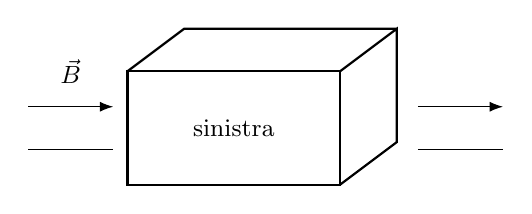
\begin{tikzpicture}[>=Latex,scale=0.9]
  \draw[thick] (0,0) rectangle (3,1.6);
  \draw[thick] (3,0)--(3.8,0.6)--(3.8,2.2)--(3,1.6) (0,1.6)--(0.8,2.2)--(3.8,2.2);
  \draw[->] (-1.4,0.5)--(-0.2,0.5) (-1.4,1.1)--(-0.2,1.1);
  \draw[->] (4.1,0.5)--(5.3,0.5) (4.1,1.1)--(5.3,1.1);
  \node[font=\small] at (-0.8,1.6) {$\vB$};
  \node[font=\small] at (1.5,0.8) {sinistra};
\end{tikzpicture}\end{center}}

\newcommand{\figdipolo}[1]{%
\begin{center}\begin{tikzpicture}[>=Latex,scale=0.9]
  \draw[->,thick,gray!60!black] (-0.3,0)--(4.2,0) node[above]{$\vB$};
  \draw[->,very thick] (0,0)--(#1:3.0) node[above right]{$\vm$};
  \draw (0.9,0) arc (0:#1:0.9) node[midway,right]{$\varphi$};
  \fill (0,0) circle (0.07);
\end{tikzpicture}\end{center}}

\newcommand{\figdipolofine}{%
\begin{center}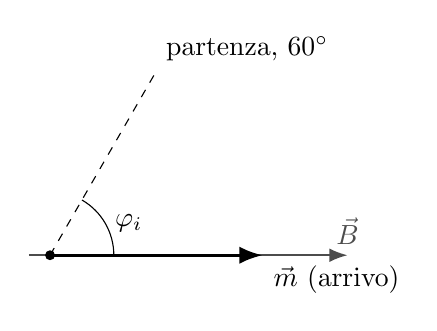
\begin{tikzpicture}[>=Latex,scale=0.9]
  \draw[->,thick,gray!60!black] (-0.3,0)--(4.2,0) node[above]{$\vB$};
  \draw[dashed] (0,0)--(60:3.0) node[above right]{partenza, $60^\circ$};
  \draw[->,very thick] (0,0)--(0:3.0) node[below right]{$\vm$ (arrivo)};
  \draw (0.9,0) arc (0:60:0.9) node[midway,right]{$\varphi_i$};
  \fill (0,0) circle (0.07);
\end{tikzpicture}\end{center}}

\newcommand{\figcurvaU}{%
\begin{center}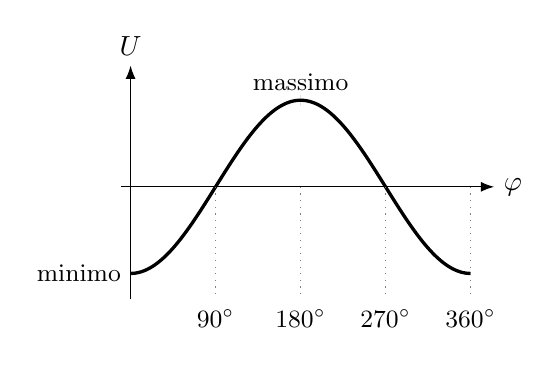
\begin{tikzpicture}[>=Latex,xscale=0.012,yscale=1.1]
  \draw[->] (-10,0)--(385,0) node[right]{$\varphi$};
  \draw[->] (0,-1.3)--(0,1.4) node[above]{$U$};
  \draw[very thick,domain=0:360,samples=73,smooth] plot (\x,{-cos(\x)});
  \foreach \x/\l in {90/$90^\circ$,180/$180^\circ$,270/$270^\circ$,360/$360^\circ$} {\draw[dotted,gray] (\x,0)--(\x,-1.3); \node[font=\small,below] at (\x,-1.3) {\l};}
  \fill (0,-1) circle (0.06) node[left,font=\small]{minimo};
  \fill (180,1) circle (0.06) node[above,font=\small]{massimo};
\end{tikzpicture}\end{center}}

\newcommand{\figcilindro}{%
\begin{center}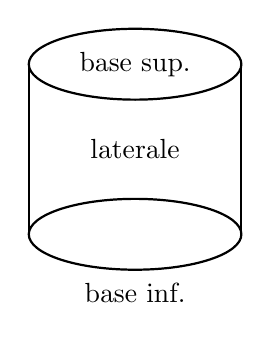
\begin{tikzpicture}[>=Latex,scale=0.9]
  \draw[thick] (0,0) ellipse (1.5 and 0.5);
  \draw[thick] (-1.5,0)--(-1.5,2.4) (1.5,0)--(1.5,2.4);
  \draw[thick] (0,2.4) ellipse (1.5 and 0.5);
  \node at (0,2.4) {base sup.};
  \node at (0,1.2) {laterale};
  \node[below] at (0,-0.55) {base inf.};
\end{tikzpicture}\end{center}}

\newcommand{\figscatola}{%
\begin{center}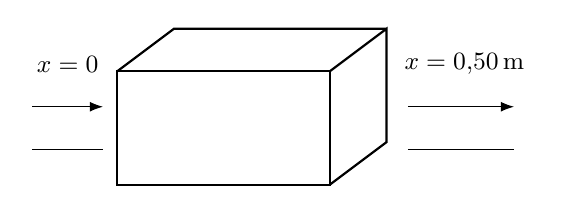
\begin{tikzpicture}[>=Latex,scale=0.9]
  \draw[thick] (0,0) rectangle (3,1.6);
  \draw[thick] (3,0)--(3.8,0.6)--(3.8,2.2)--(3,1.6) (0,1.6)--(0.8,2.2)--(3.8,2.2);
  \draw[->] (-1.2,0.5)--(-0.2,0.5) (-1.2,1.1)--(-0.2,1.1);
  \draw[->] (4.1,0.5)--(5.6,0.5) (4.1,1.1)--(5.6,1.1);
  \node[font=\small] at (-0.7,1.7) {$x=0$};
  \node[font=\small] at (4.9,1.7) {$x=0{,}50\un{m}$};
\end{tikzpicture}\end{center}}

\newcommand{\figsfere}{%
\begin{center}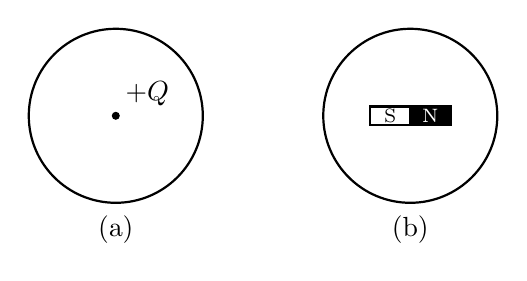
\begin{tikzpicture}[>=Latex,scale=0.85]
  \draw[thick] (0,0) circle (1.3);
  \fill (0,0) circle (0.06) node[above right]{$+Q$};
  \node at (0,-1.7) {(a)};
  \begin{scope}[xshift=4.4cm]
    \draw[thick] (0,0) circle (1.3);
    \draw[thick] (-0.6,-0.14) rectangle (0,0.14) (0,-0.14) rectangle (0.6,0.14);
    \fill (0,-0.14) rectangle (0.6,0.14);
    \node[font=\scriptsize] at (-0.3,0) {S}; \node[font=\scriptsize,white] at (0.3,0) {N};
    \node at (0,-1.7) {(b)};
  \end{scope}
\end{tikzpicture}\end{center}}

\newcommand{\figtetto}{%
\begin{center}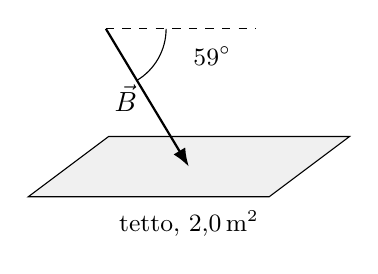
\begin{tikzpicture}[>=Latex,scale=0.85]
  \draw[fill=gray!12] (0,0)--(3.6,0)--(4.8,0.9)--(1.2,0.9)--cycle;
  \node[font=\small] at (2.4,-0.4) {tetto, $2{,}0\un{m^2}$};
  \draw[->,thick] (1.16,2.51)--(2.4,0.45) node[midway,left]{$\vB$};
  \draw[dashed] (1.16,2.51)--(3.4,2.51);
  \draw (2.06,2.51) arc (0:-59:0.9);
  \node[font=\small] at (2.75,2.1) {$59^\circ$};
\end{tikzpicture}\end{center}}

\title{\bfseries Esercizi --- Flusso di $\vB$, teorema di Gauss per il campo magnetico, dipolo in campo}
\author{4A --- 28 ottobre 2026}
\date{}

\begin{document}
\maketitle

\noindent Formule viste in classe: $\Phi_B=BS\cos\theta$ ($\theta$ angolo fra $\vB$ e la normale), $\Phi_B=0$ su ogni superficie chiusa, $\tau=mB\sin\varphi$, $U=-mB\cos\varphi$ ($\varphi$ angolo fra $\vm$ e $\vB$). Il flusso (\emph{flux}) si misura in weber, $1\un{Wb}=1\un{T\,m^2}$; il momento torcente (\emph{torque}) in $\un{N\,m}$.

\section*{Parte I --- In classe}

\needspace{16\baselineskip}\subsection*{Esercizio 1 --- Flusso attraverso una superficie piana}
\vspace{2mm}

\begin{esercizio}
\emph{Una superficie piana rettangolare di lati $20\un{cm}$ e $30\un{cm}$ è in un campo magnetico uniforme $B=0{,}40\un{T}$. Calcola il flusso di $\vB$ attraverso la superficie quando la normale alla superficie forma con $\vB$ un angolo di $0^\circ$, $60^\circ$, $90^\circ$, $180^\circ$.}
\figflusso{36}
\end{esercizio}

\begin{soluzione}
L'area è $S=0{,}20\cdot0{,}30=0{,}060\un{m^2}$ e $\Phi_B=BS\cos\theta$, con $BS=0{,}40\cdot0{,}060=2{,}4\times10^{-2}\un{Wb}$.
\begin{align*}
  \theta=0^\circ:&\quad \Phi_B=2{,}4\times10^{-2}\cdot1=2{,}4\times10^{-2}\un{Wb}=24\un{mWb}\\
  \theta=60^\circ:&\quad \Phi_B=2{,}4\times10^{-2}\cdot0{,}5=1{,}2\times10^{-2}\un{Wb}=12\un{mWb}\\
  \theta=90^\circ:&\quad \Phi_B=0\\
  \theta=180^\circ:&\quad \Phi_B=-2{,}4\times10^{-2}\un{Wb}=-24\un{mWb}
\end{align*}
A $90^\circ$ le linee ``strisciano'' lungo la superficie e non la attraversano; a $180^\circ$ la normale è opposta a $\vB$ e il flusso cambia segno.
\end{soluzione}

\bigskip\hrule\bigskip

\needspace{16\baselineskip}\subsection*{Esercizio 2 --- Il cubo e la sesta faccia}
\vspace{2mm}

\begin{esercizio}
\emph{Una superficie chiusa a forma di cubo di lato $10\un{cm}$ è in un campo magnetico non uniforme. I flussi \emph{uscenti} da cinque facce valgono $\Phi_1=+3{,}0\un{mWb}$, $\Phi_2=-5{,}0\un{mWb}$, $\Phi_3=+2{,}5\un{mWb}$, $\Phi_4=-1{,}5\un{mWb}$, $\Phi_5=+4{,}0\un{mWb}$. Quanto vale il flusso attraverso la sesta faccia? Il campo entra o esce da quella faccia?}
\figcubo
\end{esercizio}

\begin{soluzione}
La superficie è chiusa, quindi il flusso totale è nullo (Gauss per $\vB$):
\begin{align*}
  \Phi_1+\Phi_2+\Phi_3+\Phi_4+\Phi_5+\Phi_6&=0\\
  3{,}0-5{,}0+2{,}5-1{,}5+4{,}0&=+3{,}0\un{mWb}\\
  \Phi_6&=-3{,}0\un{mWb}
\end{align*}
Il flusso uscente è negativo: il campo \emph{entra} dalla sesta faccia. Il lato del cubo non serve (dato superfluo).
\end{soluzione}

\bigskip\hrule\bigskip

\needspace{26\baselineskip}\subsection*{Esercizio 3 --- Può essere un campo magnetico?}
\vspace{2mm}

\begin{esercizio}
\emph{Per ciascuna delle quattro configurazioni di linee di campo disegnate, dire se può rappresentare un campo magnetico e spiegare perché. Suggerimento: immagina una scatola chiusa attorno a una zona della figura e conta le linee che entrano e che escono.}
\figpannelli
\end{esercizio}

\begin{soluzione}
\begin{itemize}[itemsep=1pt]
  \item[(a)] \textbf{Sì}: campo uniforme; in qualunque scatola le linee che entrano sono tante quante quelle che escono.
  \item[(b)] \textbf{No}: alcune linee si interrompono nel vuoto. In una scatola chiusa attorno al punto in cui finiscono entra più flusso di quanto ne esca: $\Phi_B\neq0$, in contrasto con Gauss (le linee non finiscono mai).
  \item[(c)] \textbf{No}: le linee partono da un punto, cioè c'è una sorgente isolata (un monopolo magnetico), che non esiste.
  \item[(d)] \textbf{Sì}: linee chiuse; ogni linea entra ed esce da qualunque superficie chiusa.
\end{itemize}
\end{soluzione}

\bigskip\hrule\bigskip

\needspace{16\baselineskip}\subsection*{Esercizio 4 --- Momento torcente ed energia di un ago}
\vspace{2mm}

\begin{esercizio}
\emph{Un ago magnetico ha momento magnetico $m=0{,}80\un{A\,m^2}$ ed è in un campo uniforme $B=25\un{mT}$. Calcola il momento torcente e l'energia $U$ quando l'angolo fra $\vm$ e $\vB$ è $30^\circ$, $90^\circ$, $180^\circ$.}
\figdipolo{30}
\end{esercizio}

\begin{soluzione}
Prima si porta $B$ in tesla: $B=25\un{mT}=0{,}025\un{T}$, quindi $mB=0{,}80\cdot0{,}025=0{,}020\un{J}$ (unità: $\un{A\,m^2\,T}=\un{N\,m}=\un{J}$).
\begin{align*}
  \tau&=mB\sin\varphi: & 30^\circ&\to0{,}010\un{N\,m}, & 90^\circ&\to0{,}020\un{N\,m}, & 180^\circ&\to0\\
  U&=-mB\cos\varphi: & 30^\circ&\to-0{,}0173\un{J}, & 90^\circ&\to0, & 180^\circ&\to+0{,}020\un{J}
\end{align*}
\end{soluzione}

\bigskip\hrule\bigskip

\needspace{16\baselineskip}\subsection*{Esercizio 5 --- Equilibrio stabile o instabile?}
\vspace{2mm}

\begin{esercizio}
\emph{Guarda il grafico di $U(\varphi)=-mB\cos\varphi$. (a) In quale orientamento il momento torcente è massimo? (b) E l'energia? (c) A $180^\circ$ si ha $\tau=0$: l'equilibrio è stabile? Spiega con il grafico.}
\figcurvaU
\end{esercizio}

\begin{soluzione}
(a) Il momento torcente è massimo dove la pendenza di $U$ è massima, cioè a $90^\circ$ (e $270^\circ$), dove $\tau=mB$.\\
(b) L'energia è minima a $0^\circ$ ($U=-mB$) e massima a $180^\circ$ ($U=+mB$).\\
(c) No: a $180^\circ$ si ha $\tau=0$ ma $U$ è un \emph{massimo}. Se l'ago si sposta di poco, l'energia diminuisce, quindi il campo lo spinge ancora più lontano: equilibrio \emph{instabile} (\emph{unstable equilibrium}). $\tau=0$ non basta a dire ``stabile''.
\end{soluzione}

\bigskip\hrule\bigskip

\clearpage
\section*{Parte II --- Per casa}

\needspace{16\baselineskip}\subsection*{Esercizio 6 --- Il campo terrestre su un tetto}
\vspace{2mm}

\begin{esercizio}
\emph{In una regione il campo magnetico terrestre ha intensità $47\un{\mu T}$ ed è inclinato di $59^\circ$ sotto l'orizzontale (dati del problema). Calcola il flusso attraverso (a) un tetto piano orizzontale di area $2{,}0\un{m^2}$; (b) una parete verticale di area $2{,}0\un{m^2}$ perpendicolare alla componente orizzontale del campo.}
\figtetto
\end{esercizio}

\begin{soluzione}
(a) La normale al tetto è verticale; l'angolo fra $\vB$ e la verticale è $90^\circ-59^\circ=31^\circ$:
\[
  \Phi=BS\cos31^\circ=47\times10^{-6}\cdot2{,}0\cdot0{,}857=8{,}1\times10^{-5}\un{Wb}\approx81\un{\mu Wb}.
\]
(b) La normale alla parete è orizzontale e parallela alla componente orizzontale, $B_h=B\cos59^\circ$:
\[
  \Phi=B\cos59^\circ\cdot S=47\times10^{-6}\cdot0{,}515\cdot2{,}0=4{,}8\times10^{-5}\un{Wb}\approx48\un{\mu Wb}.
\]
\end{soluzione}

\bigskip\hrule\bigskip

\needspace{16\baselineskip}\subsection*{Esercizio 7 --- Il cilindro}
\vspace{2mm}

\begin{esercizio}
\emph{Per una superficie chiusa cilindrica, il flusso uscente attraverso la base superiore è $+8{,}0\un{mWb}$ e attraverso la superficie laterale è $-2{,}5\un{mWb}$. Calcola il flusso attraverso la base inferiore e dì se $\vB$ entra o esce.}
\figcilindro
\end{esercizio}

\begin{soluzione}
Superficie chiusa: $\Phi_{sup}+\Phi_{lat}+\Phi_{inf}=0$, quindi
\[
  \Phi_{inf}=-(8{,}0-2{,}5)=-5{,}5\un{mWb}.
\]
Il flusso uscente è negativo: $\vB$ \emph{entra} dalla base inferiore.
\end{soluzione}

\bigskip\hrule\bigskip

\needspace{16\baselineskip}\subsection*{Esercizio 8 --- Gauss per $\vec E$ e per $\vB$}
\vspace{2mm}

\begin{esercizio}
\emph{Una sfera di raggio $10\un{cm}$ racchiude: (a) una carica $+2{,}0\un{nC}$ al centro; (b) una piccola calamita. Calcola $\Phi_E$ in (a) e $\Phi_B$ in (b). Cambiano se il raggio diventa $20\un{cm}$?}
\figsfere
\end{esercizio}

\begin{soluzione}
(a) $\Phi_E=Q_{int}/\varepsilon_0=2{,}0\times10^{-9}/8{,}85\times10^{-12}=2{,}3\times10^{2}\un{N\,m^2/C}$.\\
(b) $\Phi_B=0$ per il teorema di Gauss per $\vB$.\\
Con raggio $20\un{cm}$ nulla cambia: entrambi i flussi dipendono solo da ciò che c'è dentro (la carica) o non dipendono da nulla (nessun monopolo), non dal raggio.
\end{soluzione}

\bigskip\hrule\bigskip

\needspace{16\baselineskip}\subsection*{Esercizio 9 --- Dal flusso al campo}
\vspace{2mm}

\begin{esercizio}
\emph{Una lastra piana rettangolare di area $150\un{cm^2}$, perpendicolare a $\vB$, è attraversata da un flusso di $3{,}0\un{mWb}$. Quanto vale $B$? Quanto vale il flusso se la lastra viene ruotata in modo che la normale formi $60^\circ$ con $\vB$?}
\figflusso{60}
\end{esercizio}

\begin{soluzione}
\begin{align*}
  S&=150\un{cm^2}=1{,}5\times10^{-2}\un{m^2}\\
  B&=\frac{\Phi}{S}=\frac{3{,}0\times10^{-3}}{1{,}5\times10^{-2}}=0{,}20\un{T}\\
  \Phi'&=\Phi\cos60^\circ=3{,}0\cdot0{,}5=1{,}5\un{mWb}
\end{align*}
\end{soluzione}

\bigskip\hrule\bigskip

\needspace{16\baselineskip}\subsection*{Esercizio 10 --- Quando il flusso è la metà}
\vspace{2mm}

\begin{esercizio}
\emph{Una lamina piana circolare di raggio $5{,}0\un{cm}$ è in un campo uniforme $B=0{,}20\un{T}$; la normale alla lamina forma $40^\circ$ con $\vB$. Calcola il flusso. A quale angolo il flusso vale la metà del suo valore massimo?}
\figflusso{40}
\end{esercizio}

\begin{soluzione}
\begin{align*}
  S&=\pi r^2=\pi(0{,}050)^2=7{,}85\times10^{-3}\un{m^2}\\
  \Phi_{max}&=BS=0{,}20\cdot7{,}85\times10^{-3}=1{,}57\times10^{-3}\un{Wb}\\
  \Phi&=\Phi_{max}\cos40^\circ=1{,}57\times10^{-3}\cdot0{,}766=1{,}2\times10^{-3}\un{Wb}
\end{align*}
Metà del massimo: $\cos\theta=0{,}5\Rightarrow\theta=60^\circ$.
\end{soluzione}

\bigskip\hrule\bigskip

\needspace{16\baselineskip}\subsection*{Esercizio 11 --- La scatola in campo uniforme}
\vspace{2mm}

\begin{esercizio}
\emph{Una scatola a forma di parallelepipedo è immersa in un campo uniforme $B=0{,}10\un{T}$, perpendicolare alle due facce opposte (sinistra e destra), ciascuna di area $0{,}020\un{m^2}$; $\vB$ entra dalla faccia sinistra ed esce da quella destra. Calcola il flusso uscente attraverso la faccia sinistra, la faccia destra, le altre quattro facce, e il flusso totale.}
\figscatolaB
\end{esercizio}

\begin{soluzione}
$BS=0{,}10\cdot0{,}020=2{,}0\times10^{-3}\un{Wb}$.
\begin{align*}
  \Phi_{sx}&=-BS=-2{,}0\un{mWb} &&\text{(la normale uscente è opposta a }\vB\text{)}\\
  \Phi_{dx}&=+BS=+2{,}0\un{mWb}\\
  \Phi_{4\ facce}&=0 &&(\vB\text{ è parallelo a quelle facce, }\theta=90^\circ)\\
  \Phi_{tot}&=-2{,}0+2{,}0+0=0
\end{align*}
Totale nullo, come richiede Gauss: tanto flusso entra, tanto ne esce.
\end{soluzione}

\bigskip\hrule\bigskip

\needspace{16\baselineskip}\subsection*{Esercizio 12 --- Un ago più grande}
\vspace{2mm}

\begin{esercizio}
\emph{Un ago ha $m=1{,}5\un{A\,m^2}$ ed è in un campo uniforme $B=0{,}050\un{T}$, con $\varphi=25^\circ$. Calcola $\tau$, $U$ e il lavoro esterno per ruotare l'ago da $25^\circ$ a $180^\circ$.}
\end{esercizio}

\begin{soluzione}
$mB=1{,}5\cdot0{,}050=0{,}075\un{J}$.
\begin{align*}
  \tau&=0{,}075\sin25^\circ=0{,}075\cdot0{,}423=3{,}2\times10^{-2}\un{N\,m}\\
  U&=-0{,}075\cos25^\circ=-0{,}075\cdot0{,}906=-6{,}8\times10^{-2}\un{J}\\
  W&=U(180^\circ)-U(25^\circ)=0{,}075-(-0{,}068)=0{,}143\un{J}\approx0{,}14\un{J}
\end{align*}
\end{soluzione}

\bigskip\hrule\bigskip

\needspace{16\baselineskip}\subsection*{Esercizio 13 --- Misurare $m$}
\vspace{2mm}

\begin{esercizio}
\emph{Per misurare il momento magnetico di un ago, in un campo $B=35\un{mT}$ si trova un momento torcente massimo $\tau_{max}=4{,}2\times10^{-3}\un{N\,m}$. Calcola $m$ e, per $\varphi=40^\circ$, momento torcente ed energia.}
\end{esercizio}

\begin{soluzione}
Il massimo di $\tau=mB\sin\varphi$ è $mB$ (a $90^\circ$):
\begin{align*}
  m&=\frac{\tau_{max}}{B}=\frac{4{,}2\times10^{-3}}{0{,}035}=0{,}12\un{A\,m^2}\\
  \tau(40^\circ)&=4{,}2\times10^{-3}\cdot\sin40^\circ=2{,}7\times10^{-3}\un{N\,m}\\
  U(40^\circ)&=-4{,}2\times10^{-3}\cdot\cos40^\circ=-3{,}2\times10^{-3}\un{J}
\end{align*}
\end{soluzione}

\bigskip\hrule\bigskip

\needspace{16\baselineskip}\subsection*{Esercizio 14 --- Leggere il grafico}
\vspace{2mm}

\begin{esercizio}
\emph{Un dipolo ha energia $U(\varphi)=-0{,}060\cos\varphi$ (in joule). Determina: (a) $mB$; (b) il lavoro esterno per capovolgerlo da $0^\circ$ a $180^\circ$; (c) gli orientamenti di equilibrio e la loro stabilità; (d) il momento torcente a $90^\circ$.}
\figcurvaU
\end{esercizio}

\begin{soluzione}
(a) Confrontando con $U=-mB\cos\varphi$: $mB=0{,}060\un{J}$.\\
(b) $W=2mB=0{,}12\un{J}$.\\
(c) Equilibrio a $0^\circ$ (minimo di $U$, stabile) e a $180^\circ$ (massimo, instabile): in entrambi $\tau=0$.\\
(d) $\tau(90^\circ)=mB\sin90^\circ=0{,}060\un{N\,m}$.
\end{soluzione}

\bigskip\hrule\bigskip

\needspace{16\baselineskip}\subsection*{Esercizio 15 --- Una bussola nel campo terrestre}
\vspace{2mm}

\begin{esercizio}
\emph{Una bussola ha $m=0{,}020\un{A\,m^2}$ ed è in un campo orizzontale $B=45\un{\mu T}$. Calcola il momento torcente massimo e il lavoro esterno per ruotare l'ago da $0^\circ$ a $90^\circ$ rispetto alla direzione di equilibrio.}
\end{esercizio}

\begin{soluzione}
$mB=0{,}020\cdot45\times10^{-6}=9{,}0\times10^{-7}\un{J}$.
\begin{align*}
  \tau_{max}&=mB=9{,}0\times10^{-7}\un{N\,m}\\
  W&=U(90^\circ)-U(0^\circ)=0-(-mB)=9{,}0\times10^{-7}\un{J}
\end{align*}
\end{soluzione}

\bigskip\hrule\bigskip

\needspace{16\baselineskip}\subsection*{Esercizio 16 --- Stesso prodotto $mB$}
\vspace{2mm}

\begin{esercizio}
\emph{L'ago A ha $m=0{,}40\un{A\,m^2}$ ed è in $B=10\un{mT}$; l'ago B ha $m=0{,}10\un{A\,m^2}$ ed è in $B=40\un{mT}$. Per $\varphi=30^\circ$ confronta momento torcente ed energia dei due aghi.}
\end{esercizio}

\begin{soluzione}
\begin{align*}
  mB_A&=0{,}40\cdot0{,}010=4{,}0\times10^{-3}\un{J}\\
  mB_B&=0{,}10\cdot0{,}040=4{,}0\times10^{-3}\un{J}
\end{align*}
Stesso prodotto $mB$, quindi gli stessi valori: $\tau=4{,}0\times10^{-3}\sin30^\circ=2{,}0\times10^{-3}\un{N\,m}$ e $U=-4{,}0\times10^{-3}\cos30^\circ=-3{,}5\times10^{-3}\un{J}$ per entrambi. Conta solo il prodotto $mB$, non i due fattori separatamente.
\end{soluzione}


\end{document}
